\documentclass[../../../main.tex]{subfiles}
\begin{document}
\subsection{Appendix I: DeMoivre's theorem}
\subsubsection{Example 1.} 
\begin{equation*}
    \biggl(\cos\frac{\pi}{10} + i \sin\frac{\pi}{10}\biggr)^{25} = (e^{i\pi/10})^{25} = e^{2\pi i}e^{i\pi/2} = 1 \times i = i
\end{equation*}

\subsubsection{Example 2. Find the cube roots of 8.} We write the cube roots of 8 in polar form
\begin{equation*}
    z^{1/3}=8^{1/3}e^{i(0+2n\pi)/3}
\end{equation*}
with $z=8e^{i\cdot (0+2n\pi )}$. These values are
\begin{equation*}
    \sqrt[3]{8}=2,\quad  2e^{i2\pi/3},\quad2e^{i4\pi/3}, \quad 2e^{i2\pi}, \dots
\end{equation*}
or in rectangular coordinate
\begin{equation*}
    2, \quad-1+i\sqrt{3},\quad -1-\sqrt{3}
\end{equation*}

\subsubsection{Example 3. Find and plot all values of $\sqrt[4]{-64}$.} As, before
\begin{equation*}
    z^{1/4}=64^{1/4}e^{i(\pi+2n\pi)/4}
\end{equation*}
These values are
\begin{equation*}
    \sqrt[4]{-64}=2\sqrt{2},\quad  2\sqrt{2}e^{i3\pi/4},\quad 2\sqrt{2}e^{i3\pi/4}, \quad 2\sqrt{2}e^{i5\pi/4}, \quad2\sqrt{2}e^{i7\pi/4},\dots
\end{equation*}
or in rectangular coordinate
\begin{equation*}
    \sqrt[4]{-64}=\pm 2\pm 2i
\end{equation*}

\subsubsection{Example 4. Find and plot all values of $\sqrt[6]{-8i}$}. We have uour complex number
\begin{equation*}
    z=8e^{i(1.5\pi+2n\pi)}
\end{equation*}
raised to the power of $1/6$
\begin{equation*}
    z^{1/6}=\sqrt[6]{8} e^{i(1.5\pi+2n\pi)/6}=\sqrt{2}e^{i(\pi/4+n\pi/3)}
\end{equation*}
We can do this one root at a time or more simply by using a computer to solve the equation $z^6 = -8i$.
\begin{figure*}[h]
    \centering
    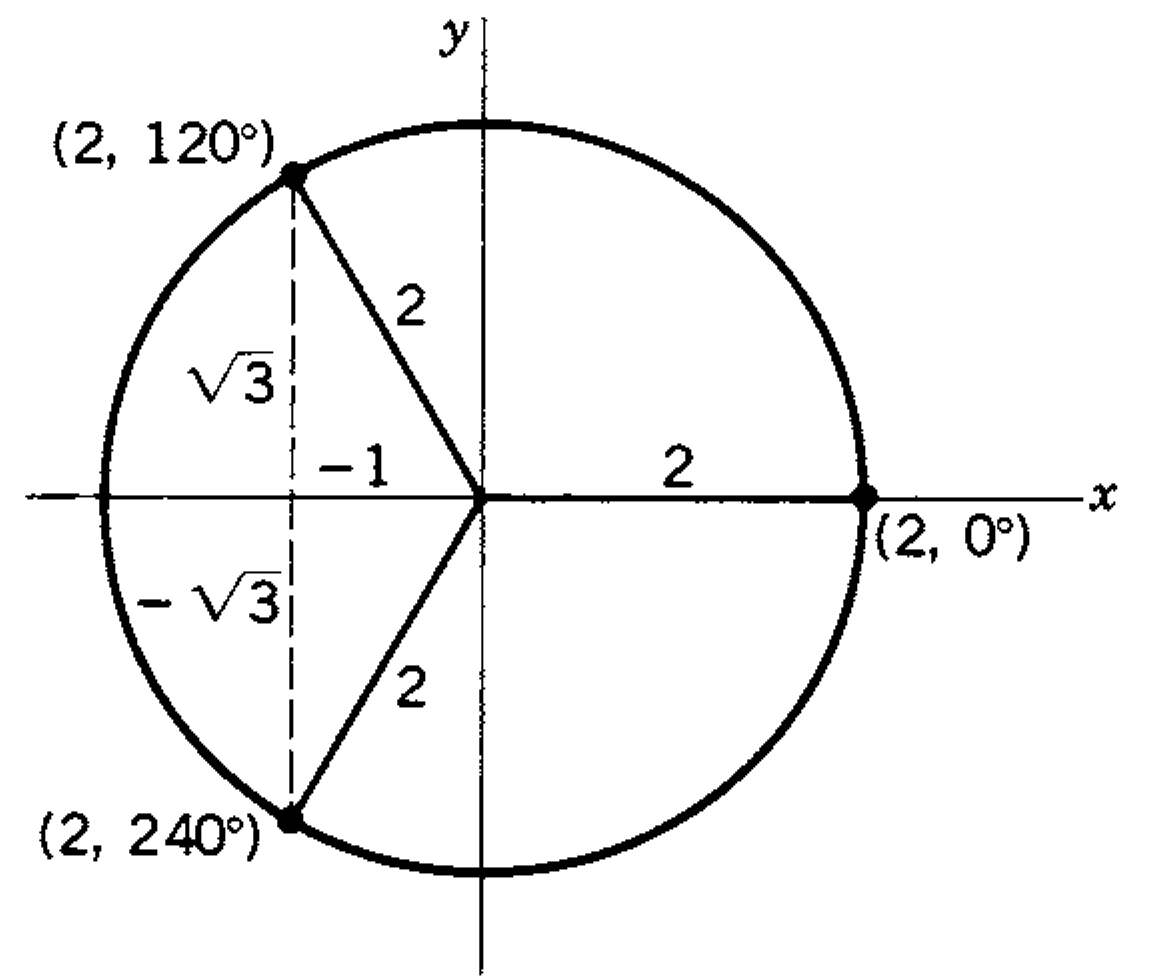
\includegraphics[width=0.3\textwidth]{../../../Rss/AnalyticsApproach/Com/AppendEx1.2.png}
    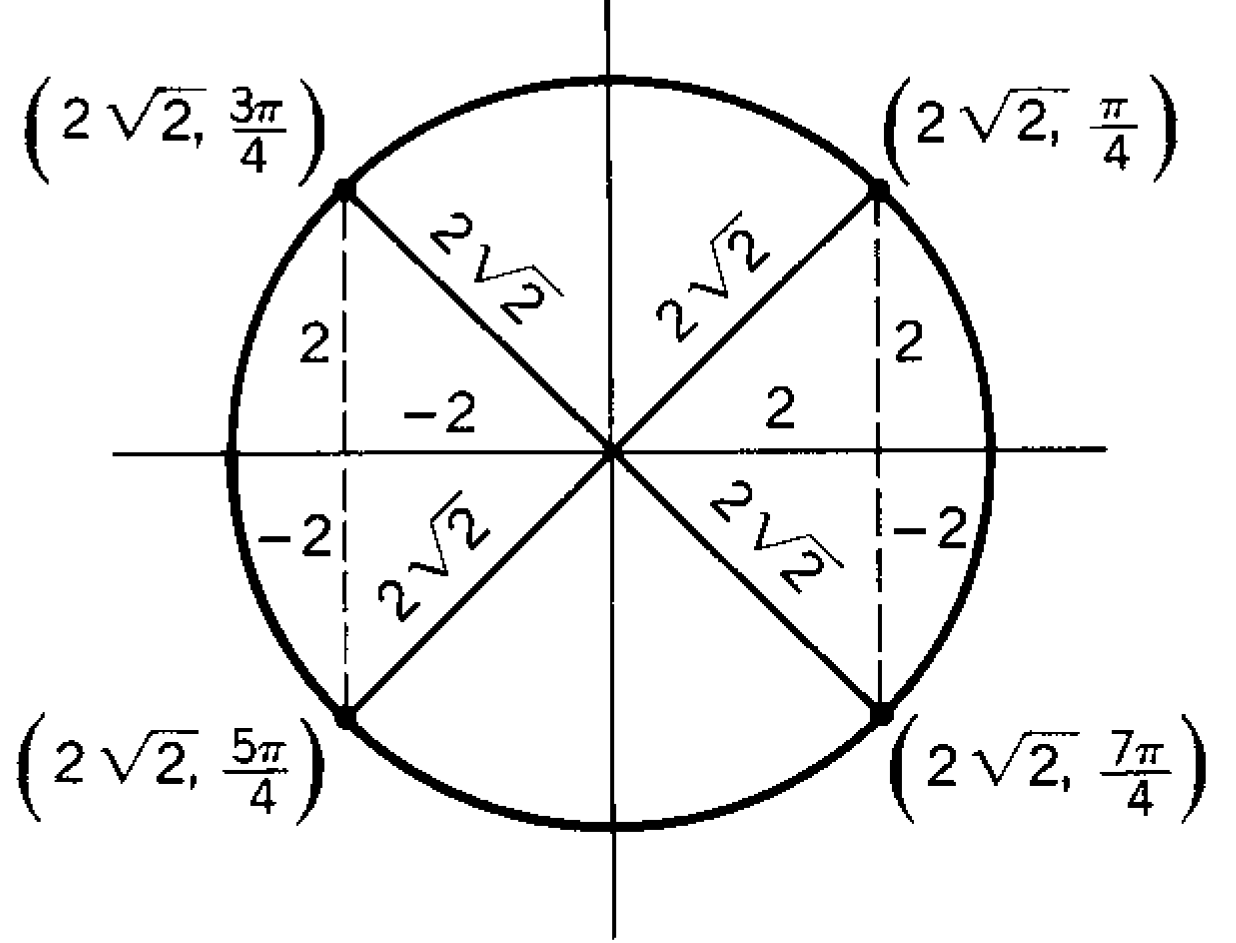
\includegraphics[width=0.3\textwidth]{../../../Rss/AnalyticsApproach/Com/AppendEx1.3.png}
    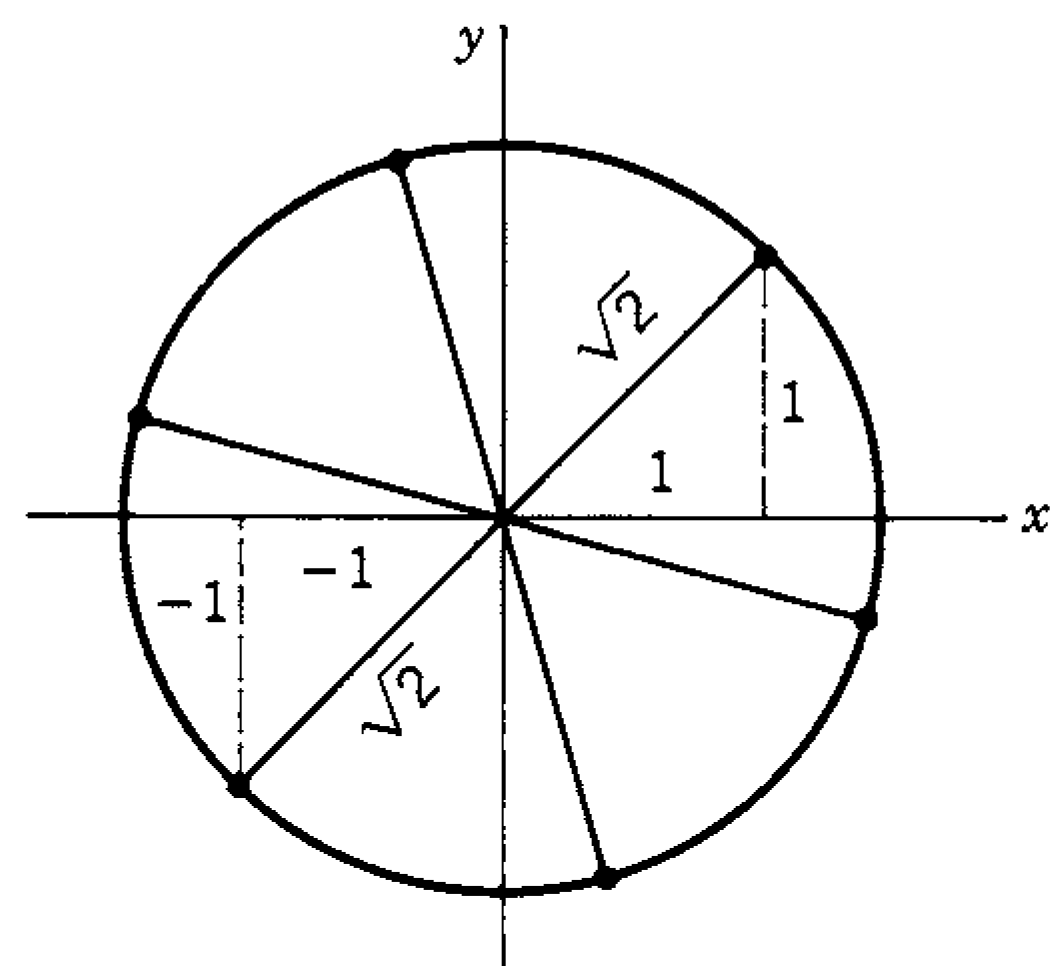
\includegraphics[width=0.3\textwidth]{../../../Rss/AnalyticsApproach/Com/AppendEx1.4.png}
    \caption*{Figure: sketch of example 2, 3 and 4}
\end{figure*} 

\subsection{Appendix II: Inverse Trigonometric} 
\subsubsection{Ex. 1: Find \emph{z} that satisfy \emph{z} = arccos 2} Since $\cos z=2$, we have
\begin{equation*}
    \frac{e^{iz}+e^{-iz}}{2}=2
\end{equation*}
To simplify the algebra, let $u = e^{iz}$ and $ u^{-1}=e^{-iz}$
\begin{equation*}
    u+u^{-1}=4
\end{equation*}
Multiply by $u$, then we get quadratic equation
\begin{equation*}
    u^2-4u+1=0
\end{equation*} 
Solving this equation
\begin{equation*}
    e^{iz}=2\pm\sqrt{3}
\end{equation*}
Take logarithms of both sides of this equation, and solve for $z$:
\begin{align*}
    iz&=\ln (2\pm\sqrt{3})+2n\pi i\\
    z&=2n\pi -i\ln (2\pm\sqrt{3})
\end{align*}

\subsubsection{Ex. 2: Evaluating Integral.} In integral tables or from your computer you may find for the indefinite integral
\begin{equation*}
    \int \frac{1}{\sqrt{x^2+a^2}}dx    =\sinh^1\frac{x}{a}
\end{equation*}
or
\begin{equation*}
    \int \frac{1}{\sqrt{x^2+a^2}}dx    =\ln\big(x+\sqrt{x^2+a^2}\big)
\end{equation*}
How are these related? Put $z=\sinh^1 x/a$, thus
\begin{equation*}
    \sinh z=\frac{x}{a}=\frac{e^z-e^{-z}}{2}
\end{equation*}
Let $e^z = u, e^{-z} = 1/u$. Then
\begin{equation*}
    au^2 - 2xu - a = 0
\end{equation*}
We solve for $u$, or rather $z$, as in the previous example
\begin{equation*}
    e^z=\frac{x\pm\sqrt{x^2-a^2}}{a}
\end{equation*}
For real integrals, that is, for real $z$, $e^z > 0$, so we must use the positive sign. Then,
taking the logarithm
\begin{equation*}
    z=\ln\big(x+\sqrt{x^2+a^2}\big)-\ln a
\end{equation*}
We see that the two answers differ only by the constant ln $a$, which is $a$ constant of integration.

\subsection{Appendix III: Laplace’s equation} 
Consider the function $u(x, y) = x^2 - y^2$. We find that
\begin{equation*}
    \nabla^2u=2-2=0
\end{equation*}that is, u satisfies Laplace’s equation (or u is a harmonic function). Let us find the
function $v(x, y)$ such that $u+iv$ is an analytic function of $z$. By the Cauchy-Riemann
equations
\begin{equation*}
    \frac{\partial u}{\partial x}=\frac{\partial v}{\partial y}=2x
\end{equation*}
Integrating partially with respect to $y$, we get
\begin{equation*}
    v(x, y) = 2xy + g(x)
\end{equation*}
where $g(x)$ is a function of $x$ to be found. Unlike our usual integration, the constant we get from partial integration not a simple constant, but rather a function of $x$.  Differentiating partially with respect to $x $ and again using the Cauchy-Riemann equations, we have
\begin{align*}
    \frac{\partial v}{\partial x}=-\frac{\partial u}{\partial y}\\
    2y+g'(x)=2y
\end{align*}
Thus we find
\begin{equation*}
    g'(x)=0\quad \text{and}\quad g(x)=C
\end{equation*}
Then
\begin{equation*}
    f(z)=x^2 - y^2 + 2ixy + C = z^2 + C
\end{equation*}
The pair of functions $u, v$ are called conjugate harmonic functions.

\subsection{Appendix IV: Residue Theorem}
\subsubsection{Ex. 1} Find \begin{equation*}
    \int_{0}^{2\pi} \dfrac{d\theta}{5+4\cos \theta}
\end{equation*}
If we make the change of variable of 
\begin{equation*}
    z = e^{i\theta}
\end{equation*}
then 
\begin{align*}
    dz &= ie^{i\theta} d\theta\\
    \cos \theta&=\frac{z+1/z}{2}
\end{align*}
As $\theta$ goes from $0$ to $2\pi$, $z$ traverses the unit circle $|z| = 1$. Making these substitutions in $I$, we get
\begin{equation*}
    I=\oint_C =\frac{dz/iz}{5+2(z+1/z)}=\frac{1}{i}\oint_C\frac{dz}{(2z + 1)(z + 2)}
\end{equation*}
where $C$ is the unit circle. The integrand has poles at $z = -1/2$ and $ z = -2$. Since only $z = -1/2$ is inside the contour $C$, the residue of the integrand is 
\begin{equation*}
    R(-1/2)=\lim_{z\rightarrow -\frac{1}{2}}(z-\frac{1}{2})\frac{1}{(2z + 1)(z + 2)}\bigg|_{z=-\frac{1}{2}}=\frac{1}{3}
\end{equation*}
Then by the residue theorem
\begin{equation*}
    I=\frac{1}{i}2\pi i R(-1/2)=\frac{2\pi}{3}
\end{equation*}

\subsubsection{Ex. 2} Evaluate \begin{equation*}
    I=\int_{-\infty}^{\infty}\frac{dx}{1+x^2}
\end{equation*}
\begin{figure*}[b]
    \centering
    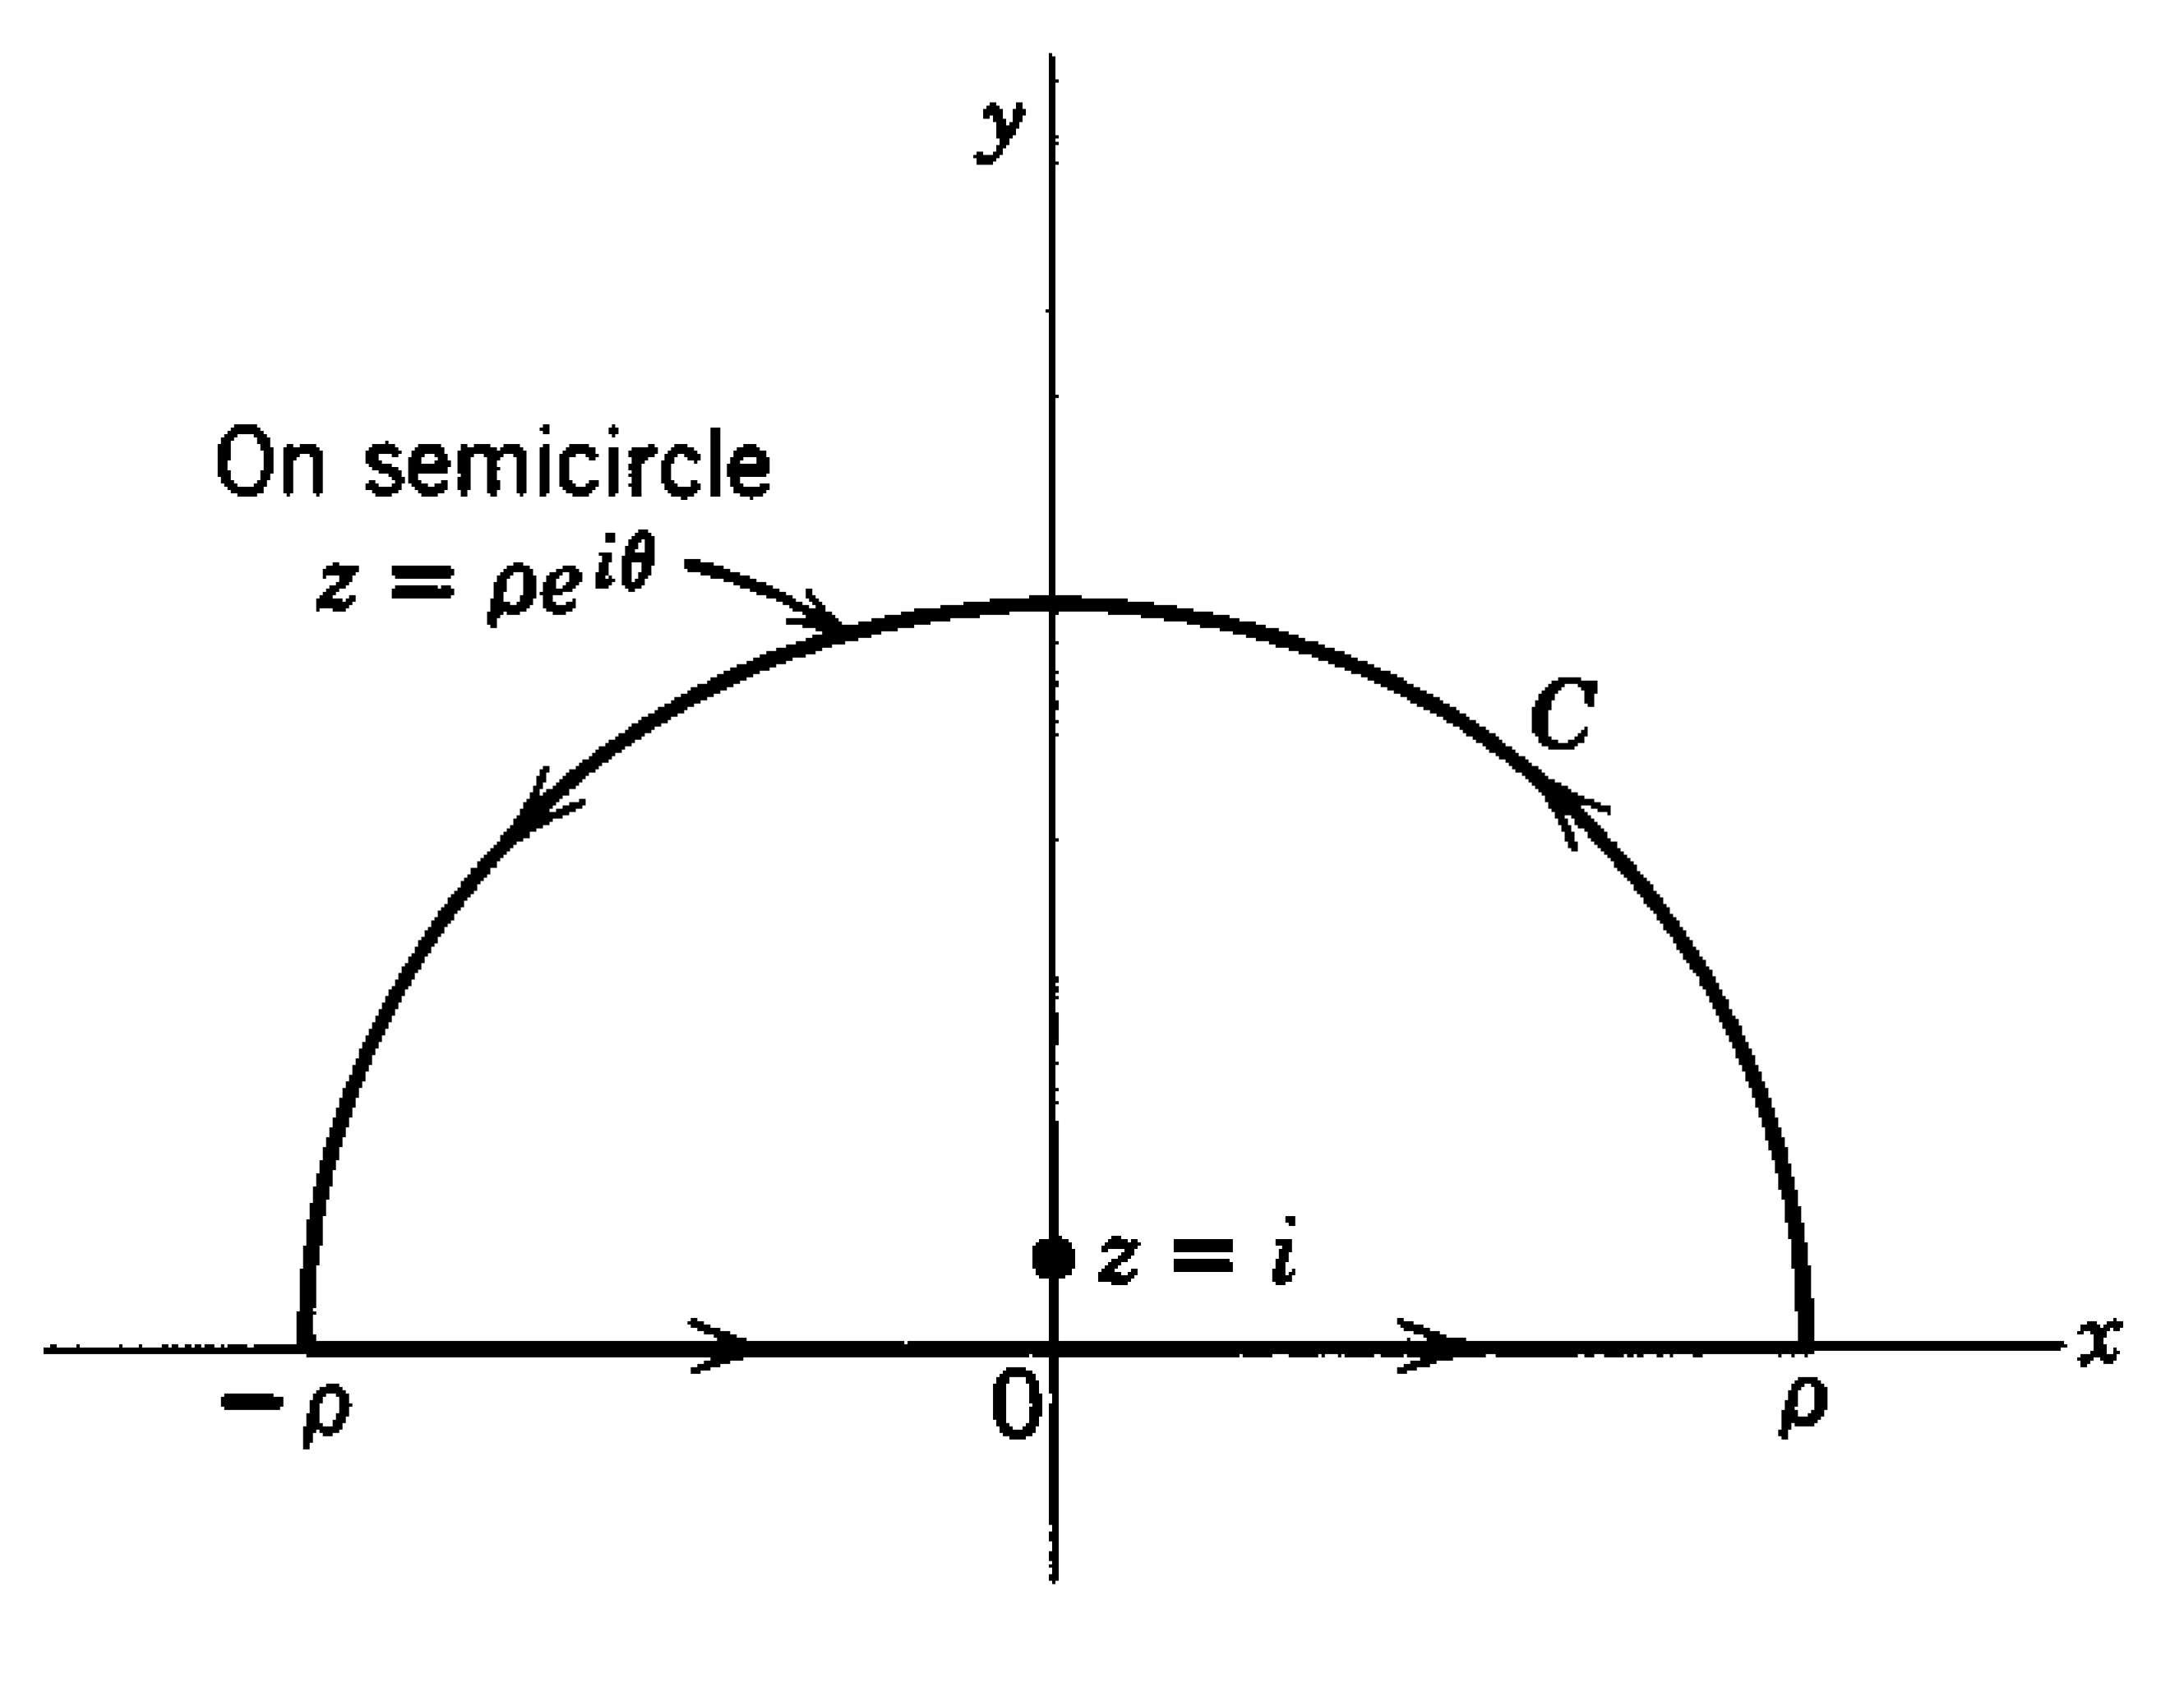
\includegraphics[width=0.5\textwidth]{../../../Rss/AnalyticsApproach/Com/Residue.png}
    \caption*{Figure: Semicircle radius $\rho$}
\end{figure*}
Altough we could evaluate $I$ by elementary method, we will use the residue theorem by considering 
\begin{equation*}
    \oint_C\frac{dz}{1+z^2}
\end{equation*}
where $C$ is the closed boundary of the semicircle with radius $\rho>1$. $C$ incloses the singular point $z = i$ and no others, thus 
\begin{equation*}
    R(i)=\lim_{z\rightarrow i}(z-i)\frac{1}{1+z^2}\bigg|_{z=i}=\frac{1}{2i}
\end{equation*}
Then the value of the contour integral is
\begin{equation*}
    I=2\pi i R(i)=\pi
\end{equation*}
Let us write the integral in two parts: (1) an integral along the $x$ axis, for this part $z = x$; (2) 
an integral along the semicircle where $z = \rho e^{i\theta}$
\begin{equation*}
    \oint_C\frac{dz}{1+z^2}=\int_{-\rho}^{\rho}\frac{dx}{1+x^2}+\int_{0}^{\pi}\frac{\rho i e^{i\theta}}{1+ \rho^2 e^{2i\theta}}d\theta=\pi
\end{equation*}
Let $\rho\rightarrow\infty$; then the second integral tends to zero since the numerator contains $\rho$ and the denominator $\rho^2$. We have 
\begin{equation*}
    \int_{-\infty}^{\infty}\frac{dx}{1+x^2}=\pi
\end{equation*}

\subsubsection{Ex. 3} Evaluate \begin{equation*}
    I =\int_{0}^{\infty}\frac{\cos x}{1+x^2}dx
\end{equation*}
We consider the contour integral
\begin{equation*}
    \oint_C\frac{e^{iz}}{1+z^2}dz
\end{equation*}
where $C$ is the same semicircular contour as before. The singular point inclosed is again $z = i$, and the residue there is
\begin{equation*}
    R(i)=\lim_{z\rightarrow i}(z-i)\frac{e^{iz}}{1+z^2}\bigg|_{z=i}=\frac{1}{2ei}
\end{equation*}
The value of the contour integral is then $\pi e$. As in before, we write the contour integral as a sum of two integrals
\begin{equation*}
    \oint_C\frac{e^{iz}}{1+z^2}dz=\int_{-\rho}^{\rho}\frac{e^{ix}}{1+x^2}dx+\int_{0}^{\pi}\frac{e^{iz}}{1+ z^2}dz=\frac{\pi}{e}
\end{equation*}
The integral along the semicircle tends to zero as the radius $\rho\rightarrow\infty$. We have then
\begin{equation*}
    \int_{-\infty}^{\infty}\frac{e^{ix}}{1+x^2}dx=\frac{\pi}{e}
\end{equation*}
Taking the real part of both sides of this equation
\begin{equation*}
    \int_{-\infty}^{\infty}\frac{\cos x}{1+x^2}dx=\frac{\pi}{e}
\end{equation*} 
Since the integrand is an even function, we have 
\begin{equation*}
    \int_{0}^{\infty}\frac{\cos x}{1+x^2}dx=\frac{\pi}{2e}
\end{equation*}

\subsubsection{Ex. 4} Evaluate
\begin{equation*}
    I=\int_{-\infty}^{\infty}\frac{\sin x}{x}dx
\end{equation*}
Here we consider
\begin{equation*}
    I=\oint \frac{e^{iz}}{z}dz
\end{equation*}
To avoid the singular point at $z = 0$, we integrate around the contour where it is on the straight line boundary. We then let the radius $r$ shrink to zero so that in effect we are integrating straight through the simple pole at the origin. Since the pole is on the straight line boundary, its contribution is just 
halfway between zero and $2\pi i\cdot$ residue.  Observing that, the integral along the large semicircle tends to zero as R tends to infinity,
\begin{figure*}[b]
    \centering
    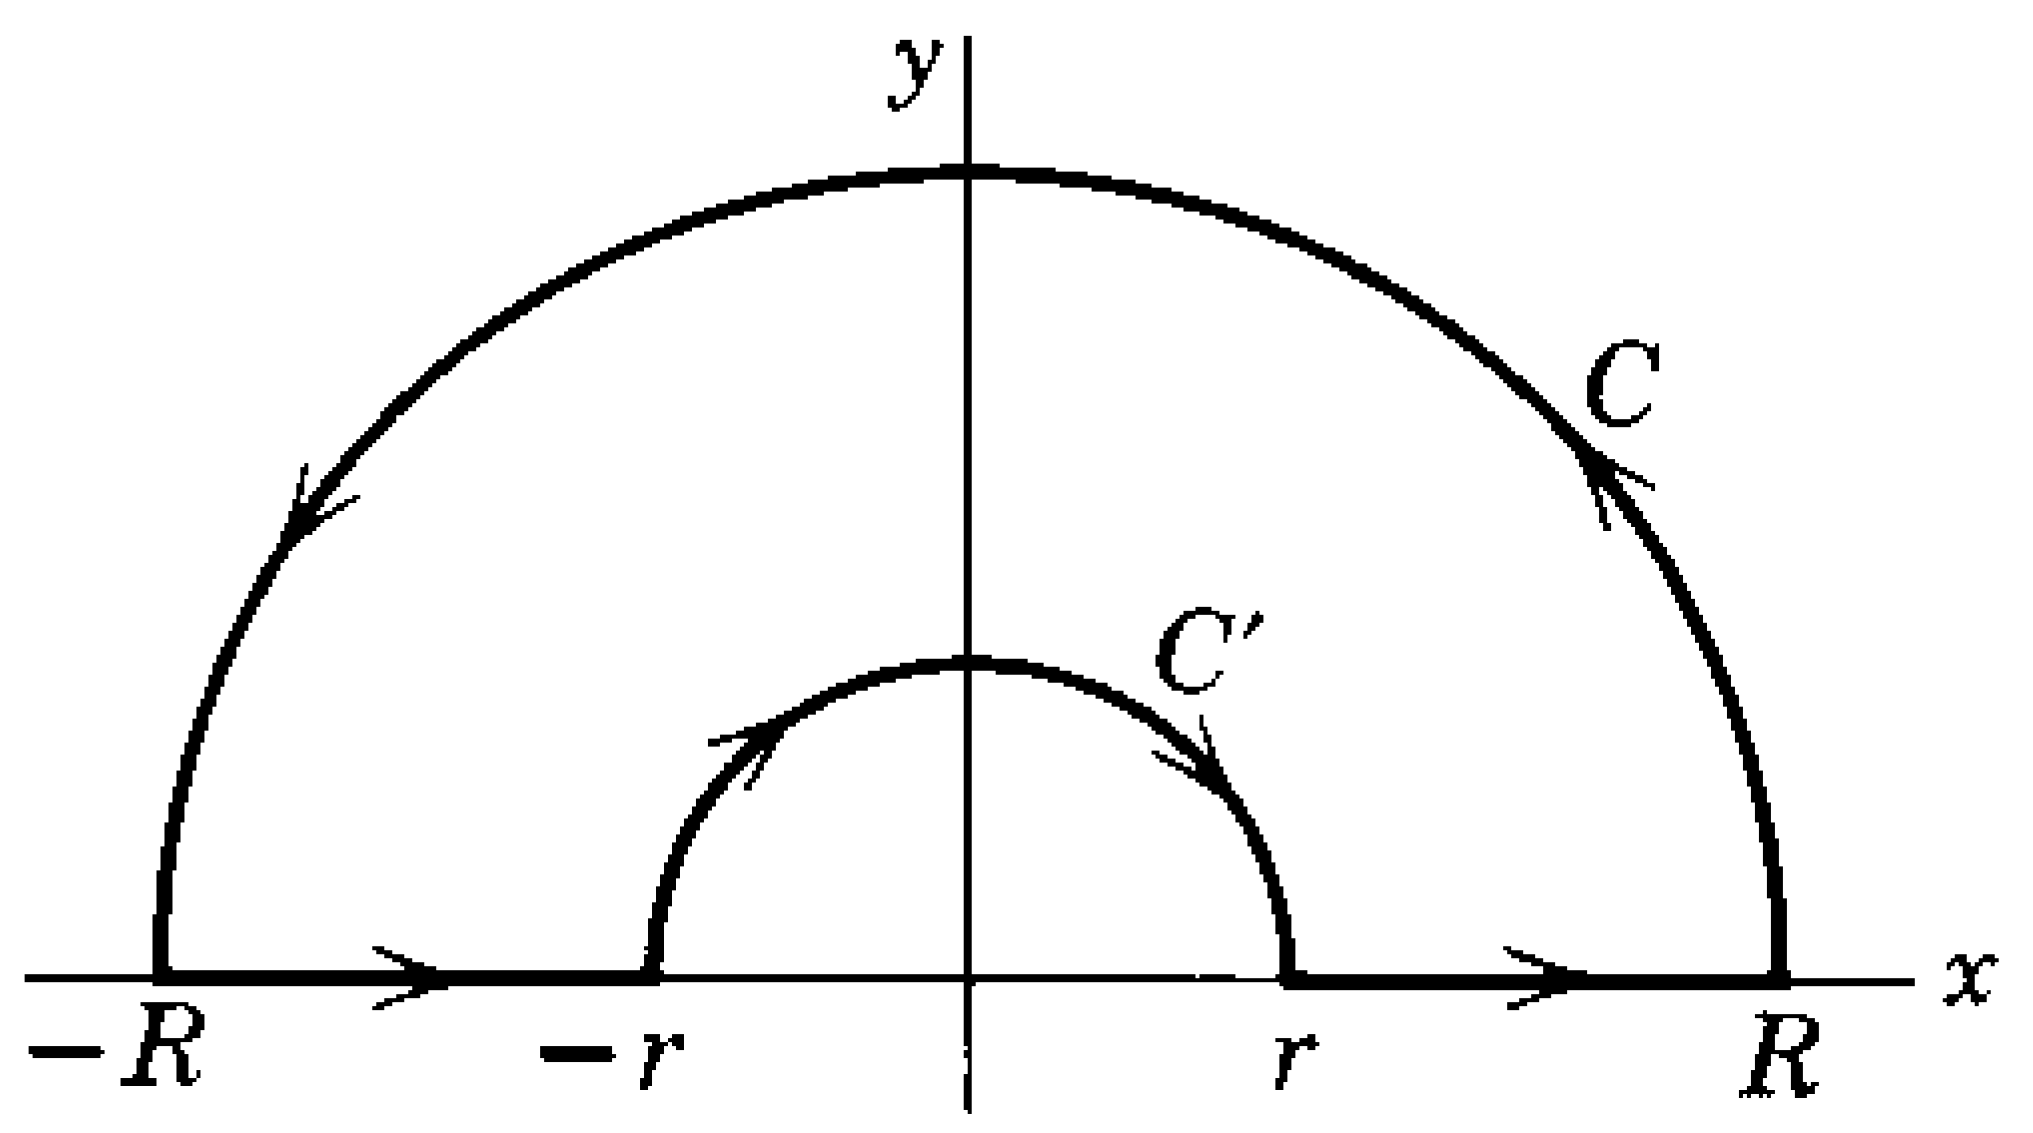
\includegraphics[width=0.5\textwidth]{../../../Rss/AnalyticsApproach/Com/Residue2.png}
    \caption*{Figure: contour of example 4}
\end{figure*}
\begin{equation*}
    I=\int_{-\infty}^{\infty} \frac{e^{ix}}{x}dx=2\pi i\cdot\frac{1}{2}R(0)=i\pi
\end{equation*}
Taking the imaginary parts of both sides, we get
\begin{equation*}
    \int_{-\infty}^{\infty} \frac{\sin x}{x}dx=\pi
\end{equation*}
\end{document}